\documentclass[a4paper,12pt,twoside]{book}
\usepackage{extra/upatras-thesis}
%
% These commands need to be defined in order to produce a correct and personalized document
%
\newcommand{\shortdoctitle}{Thesis}
\newcommand{\doctitle}{Data Search \& Extraction with Microservices}
\newcommand{\doctitlegr}{Αναζήτηση \& Εξόρυξη Δεδομένων με Microservices}
% \newcommand{\docsubtitle}{Υπότιτλος εγγράφου}
\newcommand{\division}{Electronics and Computers Department}
\newcommand{\lab}{NaN}
\newcommand{\uni}{University of Patras}
\newcommand{\unigr}{Πανεπιστήμιο Πατρών}

\newcommand{\me}{Anastasios Zampetis of Michael} %(σε γενική πτώση) ΠΡΟΣΟΧΗ: στοιχεία σε γενική πτώση. Παράδειγμα: Άγγελου Σικελιανού του Ιωάννη
\newcommand{\megr}{Αναστασίου Ζαμπέτη του Μιχαήλ} %(σε γενική πτώση) ΠΡΟΣΟΧΗ: στοιχεία σε γενική πτώση. Παράδειγμα: Άγγελου Σικελιανού του Ιωάννη
%
\newcommand{\nomme}{Anastasios Zampetis of Michael} %(σε ονομαστική πτώση) ΠΡΟΣΟΧΗ: στοιχεία σε ονομαστική πτώση. Παράδειγμα: Άγγελος Σικελιανός του Ιωάννη
%
\newcommand{\studnum}{228322}
\newcommand{\keywords}{Microservices; Data; Internet of Things; Containers}
\newcommand{\monthyear}{February 2025}

\newcommand{\supname}{Dr. Evangelos Dermatas}
\newcommand{\suptitle}{Professor}
\newcommand{\supnamegr}{Δρ. Ευάγγελος Δερματάς}
\newcommand{\suptitlegr}{Καθηγητής}

\newcommand{\cosupname}{NaN}
\newcommand{\cosuptitle}{NaN}
\newcommand{\cosupnamegr}{NaN}
\newcommand{\cosuptitlegr}{NaN}

\newcommand{\headofdivision}{Dr. George Theodoridis}
\newcommand{\headofdivisiontitle}{Assistant Professor}
\newcommand{\headofdivisiongr}{Δρ. Γεώργιος Θεοδωρίδης}
\newcommand{\headofdivisiontitlegr}{Αναπληρωτής Καθηγητής}

\author{\me}

% GLOSSARY

\makeglossaries
\setlength{\glsdescwidth}{0.7\hsize}
\setlength{\headheight}{15pt}
%\input{extra/glossary}

% BEGIN DOCUMENT
\begin{document}

% SET PAGE NUMBERING TO ROMAN
\pagenumbering{roman}
\setcounter{page}{3}

%*************************%
%         TITLES          %
%*************************%

\begin{titlepage}
\begin{center}
% Upper part of the page
{\large University of Patras - Polytechnic School}\\
\large Department of Electrical Engineering\\and Computer Technology\\
\hfill \break

\includegraphics[width= 0.8\textwidth]{up_landscape}\\
\hfill \break
{\Large Department: \division \\
Laboratory: \lab }\\[1cm]

{\uline{\LARGE{\shortdoctitle }}}\\ [0.5cm]
of the student of Department of Electrical Engineering\\
and Computer Technology of the Polytechnic School of the University of Patras\\[1cm]

{\LARGE \me }\\[0.5cm]
{\Large record number: \studnum}\\[1cm]

\uline{\large Subject}\\[0.5cm]
\textbf{\large \doctitle }\\[1cm]
\uline{\large Supervisor}\\[0.5cm]
\large \suptitle \, \supname, \uni \\[1cm]
\large{Thesis Number: }\hspace{3cm}
\vfill
% Bottom of the page
\large{Patras, \monthyear}
\end{center}
\end{titlepage}

\clearemptydoublepage

\pagestyle{empty}
\begin{center}
{\LARGE ΠΙΣΤΟΠΟΙΗΣΗ\\[1cm]}
\large Πιστοποιείται ότι η διπλωματική εργασία με θέμα\\[1cm]
\textbf{\large \doctitlegr }\\[1cm]
του φοιτητή του Τμήματος Ηλεκτρολόγων Μηχανικών και Τεχνολογίας Υπολογιστών\\[1.5cm]
\megr \\[0.5cm]
(Α.Μ.: \studnum )\\[1.5cm]
παρουσιάστηκε δημόσια και εξετάστηκε στο τμήμα  Ηλεκτρολόγων Μηχανικών και Τεχνολογίας Υπολογιστών στις\\[1cm]
\Large{\_\_/\_\_/\_\_\_}\\[1.5cm]
\end{center}
\begin{minipage}{0.5\textwidth}
\begin{flushleft} \large
Ο Επιβλέπων\\[2cm]
\supnamegr \\
\emph{\suptitlegr}\\[1cm]
% Ο Συν-Επιβλέπων\\[2cm]
% \cosupnamegr \\
% \emph{\cosuptitlegr}\\[1cm]
\end{flushleft}
\end{minipage}
\begin{minipage}{0.5\textwidth}
\begin{flushright} \large
Ο Διευθυντής του Τομέα\\[2cm]
\headofdivisiongr\\
\emph{\headofdivisiontitlegr}
\end{flushright}
\end{minipage}

\clearemptydoublepage

\pagestyle{empty}
\begin{center}
{\LARGE CERTIFICATION\\[1cm]}
\large It is certified that the Thesis with Subject\\[1cm]
\textbf{\large \doctitle }\\[1cm]
of the student of the Department of Electrical Engineering \& Computer Technology\\[1.5cm]
\me \\[0.5cm]
(R.N: \studnum )\\[1.5cm]
Was presented publicly and defended at the Department of Electrical Engineering \& Computer Technology at\\[1cm]
\Large{\_\_/\_\_/\_\_\_}\\[1.5cm]
\end{center}
\begin{minipage}{0.5\textwidth}
\begin{flushleft} \large
The Supervisor\\[2cm]
\supname \\
% \emph{\suptitle}\\[1cm]
% The Co-Supervisor\\[2cm]

\end{flushleft}
\end{minipage}
\begin{minipage}{0.5\textwidth}
\begin{flushright} \large
The Director of the Division\\[2cm]
\headofdivision\\
\emph{\headofdivisiontitle}
\end{flushright}
\end{minipage}

\clearemptydoublepage

\pagestyle{empty}
\hspace{10pt}
\begin{center}
\Large{Thesis details}\\[1cm]
{\large Subject:}
\textbf{\large \doctitle}\\[1cm]
\large {Student: \textbf{\nomme}\\[1cm]
\large{Supervising Team}\\
\textbf{\suptitle \, \supname}\\[1cm]
% \textbf{\cosuptitle \, \cosupname} \\[1cm]
% Laboratories:\\
% \lab \\[1cm]
Thesis research period:\\ December 2023 - February 2025\\[1cm]}
\end{center}

\vspace{30em}

\begin{center}
  { \large
    This thesis was written in \LaTeX.\\
  }
\end{center}


\clearemptydoublepage

\pagestyle{plain}
\begin{center}
{\LARGE Abstract}\\[1cm]
\end{center}

Microservice architecture is a widely adopted design approach in modern software development that emphasizes the development of specialized services with clearly defined capabilities and functions. This design approach has gained popularity with businesses attempting to increase responsiveness and reduce and simplify application development cycles. The improvements are realized by the integration of software engineering practices and IT operations that facilitates continuous integration, testing, and delivery, with minimal, if any, downtime. Microservices address the limitations of monolithic architectures, traditionally used in software development, by promoting modularity and independence of services. Every microservice is a separate process, and thus, development, deployment, and scaling can be achieved independently. The services may be developed with various programming languages and data storage mechanisms, thus enabling more flexibility and easy optimization. Although this model drastically improves scalability and maintainability, it requires effective orchestration and communication among the services. In today's world, vast volumes of data are being produced from various sources, such as Internet of Things (IoT) systems. However, this data is valuable only when properly processed, analysed and presented. To achieve this, technologies such as data caching, visualization, processing, and analytics are integrated into microservice-based systems. The use of these methods can enhance the amount of real-time data available, enabling and enhancing data driven decision-making in multiple sectors, such as energy management, smart cities, and industrial automation.
\clearemptydoublepage

\pagestyle{plain}
\begin{center}
{\LARGE Key Words}\\[1cm]
\end{center}

Microservices, Monolithic design, Containers, IoT, Observability, Monitoring, Synthetic Data
\clearemptydoublepage

\begin{center}
{\LARGE Acknowledgements}\\[1cm]
\end{center}

To be completed...
\clearemptydoublepage

\pagestyle{empty}

{\hypersetup{linkcolor=black}
\tableofcontents
}
\clearemptydoublepage

{\hypersetup{linkcolor=black}
\listoffigures
\listoftables
}
\glsaddall
\printglossary[style = mylong]
\printglossary[type=acronym,style=custom_acronyms]
\clearemptydoublepage

\mainmatter % book mode only
\clearemptydoublepage


\pagestyle{fancy}
\pagenumbering{arabic}
\setcounter{page}{1}

%*************************%
%       Main Chapters     %
%*************************%

% % Introduction
% \input{chapters/introduction.tex}
% \clearemptydoublepage

% Chapter 1
\chapter{Design concepts} \label{ch:design_concepts}

\section{Monolithic Architecture}

Before going into Microservices and the Microservice architecture, the Monolithic architecture approach must be explained first. The Monolithic architecture approach was till recently the preferred design option for software. In a Monolithic application all different components and functions of the business logic are combined into one indivisible program\cite{monovsmicro}. Generally these components are the user interface, business rules and data access. While individual components might be developed separately, they remain tightly coupled\cite{whatismono} and any change completed in any of them requires the whole program to be rebuild and redeployed\cite{app10175797}. More often than not development in one component requires functional changes in multiple other, adding on the development cost, complicating the build and testing process and inducing delays in deployment. A single bug in any one component can potentially halt the entire application's operation and create a nightmarish situation for on-call engineers trying to figure out the root cause and usually resulting in multiple unrelated to the issue teams joining in till root cause analysis is complete. Additionally Monolithic applications usually have large codebases, which can be cumbersome when implementing changes and difficult to manage over time\cite{whatismono}. Another major issue with Monolithic applications is scalability. Usually different components have conflicting resource requirements but because of the unified design all requirements must be handled together making scaling up the application impossible vertically, only allowing horizontal scaling through multiple copies. Scaling horizontally is very resource consuming and restricted. Finally Monolithic design allows for little to no flexibility for incorporating newer, state of the art technologies, slowly resulting in legacy applications that have to be completely redesigned and reconstructed when performance degrades. Despite the many drawbacks of Monolithic architecture, it is still favored for certain applications because of some core benefits. The most important one is performance. In most cases Monolithic applications outperform their modular counterparts\cite{whatismono}. Also initial design and implementation are easier since individual components are usually clearly defined at later stages. Additionally a single codebase and unified build and deployment process simplifies configuration management, testing and monitoring\cite{whatismono}. It is clear that the Monolithic architecture approach works well for smaller applications and helps to get things up and running faster. Furthermore when development complexity and deployment time come second to performance a Monolithic application usually has the edge over a modular approach.

\section{Microservice Architecture}

Microservices and the Microservice Architecture are, the last few years, one of the most popular design option for software applications. In the Microservice Architecture the application is structured as a collection of independent services, called Microservices. Each Microservice corresponds to a different part of the business logic, executing a well defined unique process\cite{monovsmicro}\cite{microservicesdef}. These Microservices utilize lightweight communication mechanisms, such as API interfaces, so that they can operate in unison and achieve the same final results as a Monolithic application but without being co-depended. Microservices can be build and tested separately and be deployed and scaled independently. It's Microservice should only facilitate a single function of the application and be easily comprehensible.\cite{chandrinos_thesis}. It is not hard to understand the advantages such an architecture brings compared to it's Monolithic counterpart. Each individual Microservice can be developed separately, by different teams, without compromising or delaying the development of other parts of the application. That way, different components of the application can be improved and updated asynchronously resulting in quicker deployments of the final application and the build and deployment process is straightforward and cheaper resource wise. Also, testing is incomparably easier and faster since we don't have to build and test the whole application but only a singular Microservice. Same to testing, debugging, can be quickly and effortlessly delegated to the responsible team because it is simple to pinpoint the Microservice that failed. While all these definitely play a major factor on why the Microservice Architecture is continuously gaining in popularity, the most important advantage of it is scalability. In the era of cloud native applications where being able to scale up and down on demand is of outmost importance and where costs are usage derived, Microservice based applications significantly outclass Monolithic ones. On a Microservice application scaling is possible both vertically and horizontally. If needed the whole application can be copied just like a Monolithic one but also a single Microservice can be upscaled if demand is high. More over since Microservice applications can be readily instantiated there's no need for binding resources, opposite to Monolithic application where usually at least a couple of instances need to be always up and running to cover demand spikes resulting in exponentially increased operational costs. All these advantages, thought, cannot be achieved without drawbacks. Initial development of Microservice applications requires careful and time consuming planning and design as well as a certain level of expertise since requirements and features are not yet well defined at this stage. Also Microservice applications, more often than not, lag behind Monolithic ones in performance and therefore are not suitable for time critical operations such as load balancers. Finally, Microservice architecture is not the best option for on-prem applications where customers have to setup everything manually.\cite{whenmicroarebad}

\section{Containers}

Hand in hand with the Microservice Architecture came containers. Containers are a form of virtualization similar to virtual machines (VMs), but unlike traditional virtual machines, containers share the host system's kernel while running in isolated user spaces. This architecture makes them significantly more lightweight, efficient, and versatile compared to VMs. The primary advantage of containers lies in their efficient utilization of host hardware resources and their rapid, straightforward deployment, which is ideal for scalable environments. In comparison, Vms require a separate guest operating system, adding a large overhead both resource and time wise. Consequently, compared to VMs, containers require significantly less memory and processing power, allowing for more performance out of the same hardware infrastructure.\cite{Pahl2015} Containers are spun up from images, which are built using COntainerFiles. A ContainerFile specifies a base image and a series of steps to execute on top of it, creating what are known as layers. Each step in the build process forms a new layer, which is a critical feature for development and deployment workflows, because layers are reusable, meaning that if multiple container images share common steps, those layers need to be built only once. This reuse of layers drastically reduces build time and storage space, making containerization highly compatible with agile development processes where frequent builds and deployments are common. Containers provide a consistent runtime enviroment, ensuring smooth transitions between developement, staging and production enviroments, streamlining testing and deployment process and thus minimizing release time. Efficient use of containers, especially for application deployments, require some form of orchestration. Container orchestration is usually handled through orchestration platforms, such as Kubernetes, which automates deployment, scaling and management of containerized applications ensuring high availability, resilience and insidence recovery.\cite{dockerDev}

\section{IoT device Simulators}

There's little doubt that the Internet of Things is here to stay. IoT reshaped the way humans and machines interact with the environment and is now strongly influencing most industries. In recent years more and more everyday devices are coming equipped with all sorts of sensors and internet connectivity abilities, generating big amounts of data. Along with IoT enabled devices and sensors, there's a lot of development done on IoT applications in order to make use of all the generated data and better utilize the devices. Same as all other applications, IoT apps need to be thoroughly tested before deployment to production. One way for this to be done is to create an actual IoT network of devices, specific to the application, to generate all the data and test the application. It is not hard to notice the issues with this implementation. First of all, it is very expensive to create an actual IoT network of devices, especially when there's a need to test on large ecosystems. Furthermore, it is very common for an application early in development to be redesigned and changed often and in such case IoT ecosystem used for testing will have to be redesigned and changed as well. This adds to the development cost and introduces delays to the development process. Even if an IoT network of devices is already in place for deployment reasons, testing an application using the live network can introduce security risks. Instead of using actual data from real IoT devices, synthetic data can be generated, simulating real IoT networks. 



\clearemptydoublepage

\chapter{Technologies} \label{ch:technologies}

\section{Docker}
When discussing containers, Docker cannot be left out of the discussion. Docker is an open-source platform designed to automate the creation, deployment, scaling, and management of containerized applications. It is, by far, the most widely adopted tool for containerization. Docker allows the packaging of applications and their dependencies into lightweight and easily portable containers that can be deployed consistently across a wide range of environments. This portability ensures that applications behave identically, whether running on a developer's laptop, a staging environment, or a production server.

To provision containers, Docker uses images. Docker images are read-only templates used to create containers, similar to .iso files for virtual machines, but are more lightweight and versatile. Docker images bundle everything an application needs to run, including the operating system, application code, dependencies, libraries, and configuration metadata. The metadata often includes the entry point script, a set of commands executed when the container is instantiated.

An important feature of Docker images is their layered architecture. Each layer represents a distinct change, such as adding a file, installing a package, or modifying a configuration. This layered design allows developers to build images on top of existing ones, significantly reducing build times, image sizes, and data transfer requirements.

The runtime environment responsible for building, running, and managing containers is the Docker Engine, and it consists of three main components. The first is the Docker Daemon, a background service responsible for managing Docker objects, such as containers, images, volumes, and networks. Next is the Docker Command-Line Interface (CLI), which provides a way to interact with Docker through terminal commands. Finally, the REST API enables programmatic access to Docker's functionalities.

Docker images are created using Dockerfiles, which act as blueprints for the image creation process. A Dockerfile contains step-by-step instructions for building an image, including the base image, commands to configure the environment, install dependencies, and metadata such as port configurations and the entry point script. This declarative approach ensures reproducibility, as anyone with the Dockerfile can recreate the same image, ensuring consistency across teams.

Since images are meant to be portable and used over multiple environments, remote registries to store and fetch images from are crucial. Docker Hub is a free, widely used registry provided by the wider Docker ecosystem.

Hand in hand with containers, Docker enables the creation and management of other resources critical for smooth operation. Volumes are a mechanism for persisting data generated and used by containers. Unlike ephemeral container storage, volumes ensure data remains intact even after container deletion. Docker also creates networks, enabling container interconnectivity and communication between containers and the outside world.

For handling deployments of multiple containers in a programmatic way, Docker Compose can be utilized. Docker Compose is a tool that utilizes simple YAML files to manage multi-container deployments or applications by defining services, networks, and volumes required. This approach reduces complexity and enhances reproducibility, making it easier to manage applications with multiple interconnected components.

Finally, Docker provides a native container orchestration platform, Docker Swarm, but on a production level, it is outclassed by other, more robust and feature-rich solutions, such as bare-metal Kubernetes or cloud Kubernetes services like Amazon Elastic Kubernetes Service (EKS) and Google Kubernetes Engine (GKE) that offer seamless integration and scalability.\cite{containers_docker}


\begin{figure}[!h]
    \graphicspath{ {./diagrams/} }
    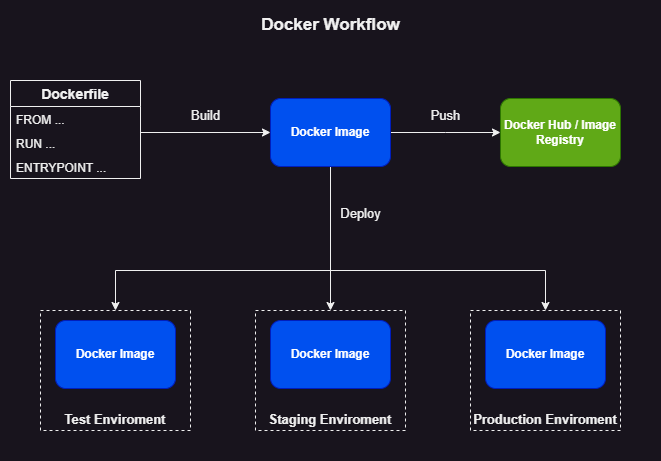
\includegraphics[scale=0.6]{docker_wf.png}
    \centering
    \caption{Docker Workflow}
    \label{fig:docker_wf}
\end{figure}

\section{Prometheus}
Prometheus is an open-source monitoring and alerting toolkit designed to provide flexible, reliable, and robust monitoring for any type of numerical data. It is considered a foundational tool for observability and a key component of modern monitoring stacks. Prometheus excels in collecting, storing, and querying time-series metrics, making it an ideal choice for monitoring infrastructure, applications, and containerized environments.

Prometheus collects and stores metrics as time-series data. Every metric is stored alongside a timestamp, allowing users to track and analyze changes over time. This feature is invaluable for identifying trends, diagnosing performance bottlenecks, and understanding long-term system behavior. Prometheus operates using a pull-based model, periodically scraping selected targets for metrics. This model ensures efficiency by fetching only the required data and enhances security by not requiring external systems to push data directly into Prometheus.

Metrics from various sources are exposed through Exporters, which transform raw data into a Prometheus-readable format. Prometheus includes a large ecosystem of pre-built exporters for common targets such as hardware systems, databases, and cloud platforms. Additionally, creating custom exporters is straightforward, making Prometheus highly adaptable to diverse use cases.

For retrieving, filtering, and manipulating time-series data, Prometheus Query Language (PromQL) is used. PromQL allows users to extract meaningful insights, create advanced visualizations, and define custom alerting rules. Prometheus also integrates seamlessly with Alertmanager, a companion tool for managing alerts. Users can define alerting rules based on PromQL expressions to trigger notifications when specific conditions, such as threshold breaches or anomalies, are met. Alertmanager routes these alerts to appropriate channels, such as email, Slack, or webhooks.

For short-lived jobs that may terminate before Prometheus can scrape their metrics, the PushGateway provides a solution. This intermediary gateway allows these jobs to push metrics temporarily, ensuring no data loss. Prometheus also supports Service Discovery, enabling automatic detection of scrape targets in dynamic environments like Kubernetes. This eliminates the need for manual configuration, making it ideal for large-scale, constantly changing systems.

Prometheus employs a highly optimized, custom-built database for storing time-series data. This database supports fine-grained retention policies, allowing users to define which metrics to retain and for how long, thereby optimizing storage usage. Prometheus further enhances usability with its ability to label metrics using key-value pairs. These labels provide additional context and facilitate filtering and aggregation, enabling multidimensional analysis of metrics.

Although Prometheus offers basic visualization capabilities, it integrates natively with Grafana, the industry-leading visualization platform. This integration allows users to build interactive, feature-rich dashboards. While Prometheus is optimized for metrics collection, it is not suitable for other types of data, such as logs. To complement Prometheus, tools like Loki are often used to handle log data, creating a comprehensive observability stack.\cite{Jani2024-mg,Pragathi2024-fa}



\section{Grafana}
Usually, when utilizing Prometheus to gather metrics, Grafana is employed as the visualization tool of choice. Grafana is an open-source platform for monitoring and observability, designed to enable users to visualize, query, and analyze data from an extensive range of data sources. By transforming raw metrics into actionable insights, Grafana facilitates the creation of complex, interactive dashboards, making it an essential component of most modern monitoring and observability implementations.

These dashboards are highly customizable, combining a diverse variety of visualizations, such as line graphs, heatmaps, gauges, tables, and single-stat panels. This flexibility allows teams to represent various types of information, including historical data, real-time system statuses, and long-term trends, in a visually appealing and intuitive manner.

Grafana supports integration with a broad array of data sources, including Prometheus, Loki, PostgreSQL, MySQL, and cloud services. Its ability to query multiple sources simultaneously enables advanced, multifaceted analyses, where data from disparate systems can be combined and manipulated for deeper insights.

Grafana also has support for variable creation, which allows users to dynamically assign values from the sourced data. This capability enables the construction of dynamic dashboards with parameterized views that adapt to different environments, datasets, or conditions without requiring additional customization. Such dynamic behavior unlocks templating, where reusable dashboards can be developed, significantly enhancing efficiency and consistency across monitoring setups.

Grafana excels at centralizing observability, providing a unified view of the health and performance of systems, services, and applications. Its real-time visualizations empower teams to detect and address issues as they emerge, enabling faster response times and minimizing downtime.

At the same time, the ability to chart and analyze historical data enables the identification of recurring trends and the prediction of potential problems, thus allowing the implementation of proactive measures to mitigate risks.

Lastly, Grafana offers alerting capabilities, same as Prometheus with Alertmanager, that can push notifications on various channels when a set of conditions is met\cite{grafana, promandgraf}.

\begin{figure}[!h]
    \graphicspath{ {./diagrams/} }
    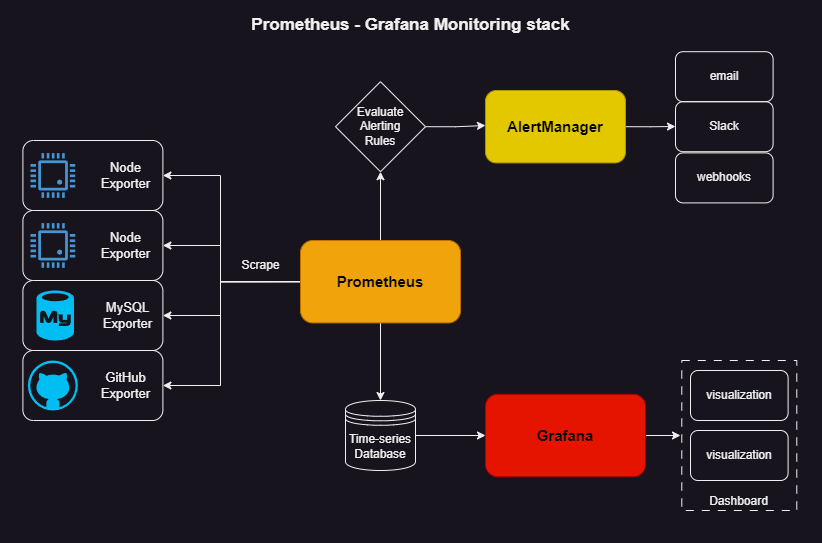
\includegraphics[scale=0.55]{prom-graf.png}
    \centering
    \caption{Prometheus-Grafana Monitoring stack}
    \label{fig:prom_graf}
\end{figure}

\section{Message Queuing Telemetry Transport (MQTT)}
Message Queuing Telemetry Transport (MQTT) is a lightweight, publish/subscribe model messaging protocol specifically designed for devices with limited computational resources and unreliable, low-bandwidth networks. Its efficiency and reliability make it a standard choice for IoT device communication and similar constrained environments.

At its core, MQTT operates using the publish/subscribe model, a decoupled communication architecture where publishers (senders) and subscribers (receivers) exchange messages through a central broker. The MQTT broker serves as the backend system responsible for managing message coordination between clients. Its key responsibilities include receiving and filtering messages, identifying clients subscribed to specific topics, and forwarding messages to those subscribers. Popular MQTT brokers are EMQX, HiveMQ and Mosquitto. Mosquitto was preferred in this implementation for it's lightweight nature, which fits well in a microservice approach.

In typical communication, MQTT clients (which can act as publishers, subscribers, or both) establish a connection with the broker using an MQTT connection. The broker confirms the connection, ensuring both entities are ready to exchange messages. MQTT requires a TCP/IP stack on both clients and brokers for communication, and clients never connect directly with each other but only with the broker. Once connected, the client can either publish messages, subscribe to specific messages, or do both. The broker filters incoming messages using topics, which are structured hierarchically, similar to folder directories in a filesystem. The broker only sends messages to subscribers from the topics they have explicitly subscribed to.

The MQTT protocol is widely regarded as a standard for IoT data transmission and for good reason. Firstly, it requires minimal hardware resources, so it can even be used by small battery-powered microcontrollers. MQTT control messages and MQTT message headers are quite small, reducing network overhead and ensuring efficient use of bandwidth. MQTT has build-in features like quick device reconnections and quality-of-service (QoS) levels, which ensure reliable message delivery even on the unreliable, low-bandwidth and high latency cellular networks IoT devices usually operate on. The decouple nature of MQTT, combined with the low bandwidth requirements allows it to easily handle large number of clients, making it very scalable. 

Despite its many strengths, MQTT does have a few limitations. The broker acts as the central node, and subsequently as a single point of failure, so any disruption or failure of the broker results in a complete communication breakdown. This risk can be mitigated through high-availability setups. Also the maximum payload is 256MB and large payloads can impact performance but in an IoT scenario. However, such large payloads are uncommon. Lastly, MQTT lacks native encryption but modern authentication protocols such as OAuth and TLS can be easily integrated\cite{mqtt}.

\begin{figure}[!h]
    \graphicspath{ {./diagrams/} }
    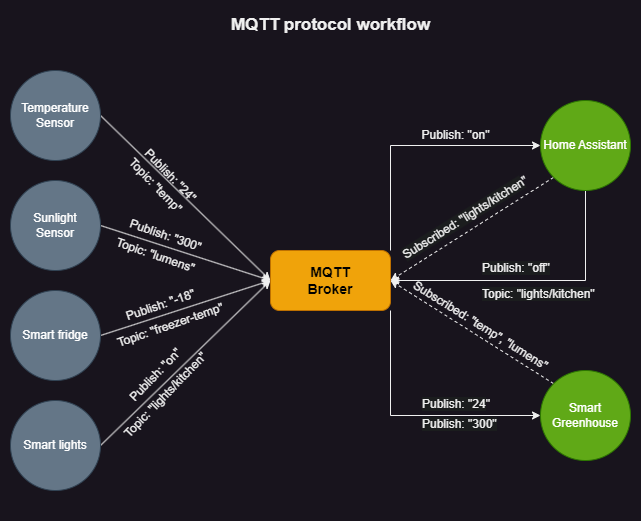
\includegraphics[scale=0.7]{mqtt.png}
    \centering
    \caption{MQTT protocol workflow}
    \label{fig:mqtt}
\end{figure}
\clearemptydoublepage

\chapter{Implementation} \label{ch:implementation}

\section{Design and Architecture}
The design of the implementation leverages a microservices architecture to simulate real-world data collection and processing. The system was designed to emulate a sensor-driven environment, utilizing containerized services for data generation, communication, transformation, and visualization.

To simulate real sensors or microcontrollers, a python application was developed. This application processes a real dataset of air quality data and extracts the data corresponding to specific timestamps. The extracted data is then published to an MQTT broker. This python application is packaged in a Docker image to enable scalability and reusability. Multiple instances of this sensor simulation image are deployed as separate Docker containers, each simulating an independent sensor.

To enable communication using the MQTT protocol between the simulated sensors and the data-processing layer, an MQTT broker was deployed. The MQTT broker, also packaged in a Docker container, receives data from the sensor containers and forwards it to the subscribed clients.

A controller service was implemented as a Python application. This application subscribes to the MQTT topics published by the sensors, processes the incoming data, and converts it into a format compatible with Prometheus. The transformed data is then exposed through an HTTP endpoint. The controller application is also containerized and deployed as a separate Docker container.

Prometheus was deployed in a Docker container and configured to periodically scrape the data exposed by the controller service and to retain it for an appropriate amount of time.

Finally, Grafana was deployed as the visualization layer of the system, again in its own Docker container. Grafana was configured to use Prometheus as its data source. Custom dashboards were created to visualize the air quality data collected from the simulated sensors, enabling real-time monitoring and analysis.

The entire system was deployed using Docker Compose to allow for a easy orchestration and management of all the containerized services and for a straightforward, scalable and reproducible deployment.

\begin{figure}[!h]
    \graphicspath{ {./diagrams/} }
    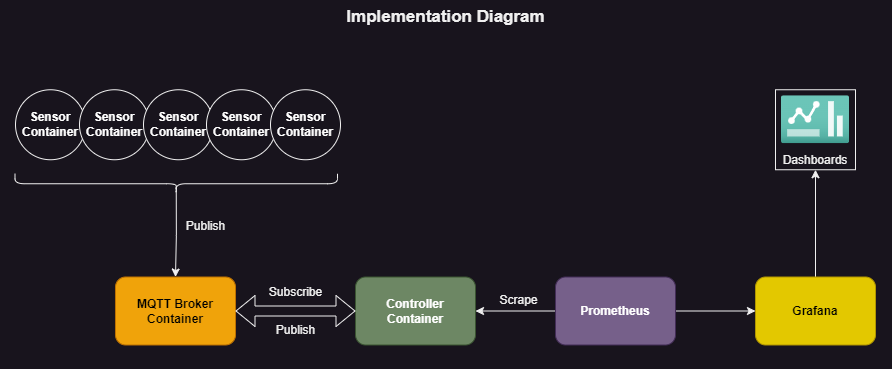
\includegraphics[scale=0.55]{implementation.png}
    \centering
    \caption{Implementation Diagram}
    \label{fig:imple_dia}
\end{figure}

\section{Dataset}
\subsection{Dataset Description}
The dataset used contains the responses of a gas multisensor device deployes on the field in an Italian city. Hourly responses averages are recorded along with gas concentrations references from a certified analyzer. The dataset contains 9357 instances of hourly averaged responses from an array of 5 metal oxide chemical sensors embedded in an Air Quality Chemical Multisensor Device. Ground Truth hourly averaged concentrations for CO, Non Metanic Hydrocarbons, Benzene, Total Nitrogen Oxides (NOx) and Nitrogen Dioxide (NO2) were provided by a co-located reference certified analyzer. Dataset can be found \href{https://www.kaggle.com/datasets/fedesoriano/air-quality-data-set/data}{here}.

\begin{table}[!h]
\begin{tabular}{|c|p{0.8\linewidth}|}
    \hline
    \multicolumn{2}{|c|}{\textbf{Attribute Information}} \\
    \hline
    \hline
    0& Date (DD/MM/YYYY) \\ \hline
    1& Time (HH.MM.SS) \\ \hline
    2& True hourly averaged concentration CO in $mg/m^3$ (reference analyzer) \\ \hline
    3& PT08.S1 (tin oxide) hourly averaged sensor response (nominally CO targeted) \\ \hline
    4& True hourly averaged overall Non Metanic HydroCarbons concentration in $microg/m^3$ (reference analyzer) \\ \hline
    5& True hourly averaged Benzene concentration in $microg/m^3$ (reference analyzer) \\ \hline
    6& PT08.S2 (titania) hourly averaged sensor response (nominally NMHC targeted) \\ \hline
    7& True hourly averaged NOx concentration in ppb (reference analyzer) \\ \hline
    8& PT08.S3 (tungsten oxide) hourly averaged sensor response (nominally NOx targeted) \\ \hline
    9& True hourly averaged NO2 concentration in $microg/m^3$ (reference analyzer) \\ \hline
    10& PT08.S4 (tungsten oxide) hourly averaged sensor response (nominally NO2 targeted) \\ \hline
    11& PT08.S5 (indium oxide) hourly averaged sensor response (nominally O3 targeted) \\ \hline
    12& Temperature in °C \\ \hline
    13& Relative Humidity (\%) \\ \hline
    14& AH Absolute Humidity  \\ \hline
\end{tabular}
\centering
\caption{Dataset Attribute Information}
\label{fig:dataset_attri}
\end{table}

\subsection{Dataset Manipulation}
Dataset was originally formatted in comma-separated values (CSV) format to be easily imported in a spreadsheet. To bring the CSV formatted dataset in a programmatically friendlier json format, a python script was developed. 
To assist with the randomized nature of data generation by the sensor simulator, for every timestamp a json object was created, with key an incremental integer and value the collection of metrics in json object format. Also empty rows were removed.

\begin{minted}[%
    framesep=2mm,
    baselinestretch=1.2,
    bgcolor=LightGray,
    fontsize=\footnotesize,
    breaklines
    ]{python}
    import csv
    import sys
    import json
    import os

    # Creates a new csv file named 'edited_csv' that doesn't contain empty rows, or rows with empty fields
    def csv_cleanup(csvfilename):
        with open(csvfilename, newline='') as csvfile:
            with open('edited_csv', 'w', newline='') as edited_csvfile:
                original = csv.reader(csvfile, delimiter=';')
                edited = csv.writer(edited_csvfile, delimiter=';')
                # fieldnames = next(original)
                # fieldnames.insert(0, "#")
                # edited.writerow(fieldnames)
                # i = 1
                for row in original:
                    if row and any(row) and any(field.strip() for field in row):
                        # row.insert(0, i)
                        edited.writerow(row)
                        # i += 1

    # Creates a json file from the edited csv file with an incremental integer as keys
    def csv_to_json(filename):
        data_dict = {}
        with open('edited_csv', newline='') as csvfile:
            edited = csv.DictReader(csvfile, delimiter=';')
            key = 1
            for row in edited: 
                data_dict[key] = row
                key += 1
        with open(filename+'.json', 'w') as jsonfile:
            jsonfile.write(json.dumps(data_dict, indent = 4))



    csvfilename = sys.argv[1]
    filename = csvfilename.split('/')[-1].split('.')[0]

    csv_cleanup(csvfilename)
    csv_to_json(filename)
    os.remove('edited_csv')
\end{minted}

The json re-formated dataset is structured as seen below.

\begin{minted}[%
    framesep=2mm,
    baselinestretch=1.2,
    bgcolor=LightGray,
    fontsize=\footnotesize,
    breaklines
    ]{json}
    {
        "1": {
            "Date": "10/03/2004",
            "Time": "18.00.00",
            "CO(GT)": "2,6",
            "PT08.S1(CO)": "1360",
            "NMHC(GT)": "150",
            "C6H6(GT)": "11,9",
            "PT08.S2(NMHC)": "1046",
            "NOx(GT)": "166",
            "PT08.S3(NOx)": "1056",
            "NO2(GT)": "113",
            "PT08.S4(NO2)": "1692",
            "PT08.S5(O3)": "1268",
            "T": "13,6",
            "RH": "48,9",
            "AH": "0,7578",
            "": ""
        },
        "2": {
            "Date": "10/03/2004",
            "Time": "19.00.00",
            "CO(GT)": "2",
            "PT08.S1(CO)": "1292",
            "NMHC(GT)": "112",
            "C6H6(GT)": "9,4",
            "PT08.S2(NMHC)": "955",
            "NOx(GT)": "103",
            "PT08.S3(NOx)": "1174",
            "NO2(GT)": "92",
            "PT08.S4(NO2)": "1559",
            "PT08.S5(O3)": "972",
            "T": "13,3",
            "RH": "47,7",
            "AH": "0,7255",
            "": ""
        }
    }
\end{minted}

\section{Sensor Simulator}
\subsection{Scenario}
The sensors remain in a low-power idle state to conserve energy. They are subscribed to the "collect-data" topic but are not actively collecting or publishing data. The controller node publishes a message to the MQTT topic "collect-data". This message is broadcast to all subscribed sensors by the MQTT broker. Upon receiving the trigger from the collect-data topic, sensors begin collecting air quality metrics. After collecting the data, each sensor publishes its metrics to its respective MQTT topic and returns to an idle state.
\subsection{Application}
As described on the scenario, first action on the application is establishing a connection to the MQTT broker, making sure to reconnect in case of disconnection, which would happen often in a real case scenario utilizing an unreliable cellular connection and subscribing to the "collect-data" topic. Then, once a message from the topic is received the data collection and publishing script is executed.

\begin{minted}[%
    framesep=2mm,
    baselinestretch=1.2,
    bgcolor=LightGray,
    fontsize=\footnotesize,
    breaklines
    ]{python}
    import socket
    import time
    import subprocess
    import paho.mqtt.client as mqtt_client

    port = 1883  # Default port for MQTT communication
    topic = "collect-data"  # Topic to subscribe to for data collection
    hostname = socket.gethostname()  # Get the hostname of the machine running this script. Machine (container) hostname is enforced later-on by docker compose 
    client_id = 'subscribe-{}'.format(hostname)  # Unique client ID for MQTT connection
    # broker = 'localhost'  # Uncomment this line for local broker testing
    broker = 'host.docker.internal'  # Use when running in a Docker environment

    def connect_mqtt():
        """
        Connects to the MQTT broker and sets up event handlers for connect, disconnect, and message events.
        """

        def on_connect(client, userdata, flags, rc):
            """
            Callback triggered upon connecting to the MQTT broker.
            """
            if rc == 0:
                print("Connected to MQTT Broker!")
                client.subscribe(topic)  # Subscribe to the specified topic
            else:
                print("Failed to connect, return code %d\n", rc)
        
        def on_disconnect(client, userdata, rc):
            """
            Callback triggered when the MQTT client disconnects from the broker.
            Implements an exponential backoff strategy for reconnection attempts.
            """
            FIRST_RECONNECT_DELAY = 1
            RECONNECT_RATE = 2
            MAX_RECONNECT_COUNT = 12
            MAX_RECONNECT_DELAY = 60

            print("Disconnected with result code: %s", rc)
            reconnect_count, reconnect_delay = 0, FIRST_RECONNECT_DELAY
            while reconnect_count < MAX_RECONNECT_COUNT:
                print("Reconnecting in {} seconds...".format(reconnect_delay))
                time.sleep(reconnect_delay)

                try:
                    client.reconnect()
                    print("Reconnected successfully!")
                    return
                except Exception as err:
                    print("{}. Reconnect failed. Retrying...".format(err))

                reconnect_delay *= RECONNECT_RATE
                reconnect_delay = min(reconnect_delay, MAX_RECONNECT_DELAY)
                reconnect_count += 1
            print("Reconnect failed after {} attempts. Exiting...".format(reconnect_count))

        def on_message(client, userdata, msg):
            """
            Callback triggered when a message is received on the subscribed topic.
            """
            print("Received `{}` from `{}` topic".format(msg.payload.decode(), msg.topic))
            subprocess.run(["./sensor_data"])  # Execute the sensor_data script upon message receipt

        # Create an MQTT client instance, assign the callback functions and connect
        client = mqtt_client.Client(client_id)
        client.on_connect = on_connect
        client.on_disconnect = on_disconnect
        client.on_message = on_message
        client.connect(broker, port)
        return client  # Return the configured client instance

    def run():
        """
        Main function to connect the MQTT client and start its loop.
        """
        client = connect_mqtt()
        client.loop_forever()

    if __name__ == '__main__':
        run()
\end{minted}

The data collection script, again starts by establishing a connection client with the MQTT broker. Once connection is established, the data collection process starts. To simulate a real-world scenario, to add variation between the multiple sensors and a randomization element, that also prolongs the use of the dataset before going over the same data, an elaborate process was devised. To ensure the randomized data have a real-world, logical flow, the next data point is selected from the range (previous - 2, previous + 3). This ensures that the metrics collected each time are only a few hours apart instead of completely random, which would result in completely abnormal differences on metrics that wouldn't be observed on metrics taken a few minutes or an hour apart. It also ensures that the data point slowly moves forward in time, as to not overly repeat the same data. The starting point for this process is randomized using another script, to ensure results between sensors don't overlap heavily. Since the data collection process is ephemeral, the data points needs to be stored. This could have been achieved in a number of ways, like passing it back and forth between the main subscription script or using an environmental variable, but storing to a file was preferred as it could also be utilized if a recovery scenario was to be covered. Once the end of the database is reached, a new starting point is, again, randomly selected.

\begin{minted}[%
    framesep=2mm,
    baselinestretch=1.2,
    bgcolor=LightGray,
    fontsize=\footnotesize,
    breaklines
    ]{python}
    import json
    import random, os
    import socket
    import subprocess
    from dotenv import load_dotenv
    import paho.mqtt.client as mqtt_client

    port = 1883  # Default port for MQTT communication
    hostname = socket.gethostname()  # Retrieve the hostname of the current machine. Hostname is enforced by docker compose.
    topic = "sensor-data/{}".format(hostname)  # Define the unique topic for publishing sensor data
    client_id = 'publish-{}'.format(hostname)  # Unique client ID for MQTT connection
    # broker = 'localhost'  # Uncomment this line for local broker testing
    broker = 'host.docker.internal'  # Use this broker when running in a Docker environment

    def connect_mqtt():
        """
        Connects to the MQTT broker and sets up the on_connect callback.
        """

        def on_connect(client, userdata, flags, rc):
            """
            Callback triggered upon connecting to the MQTT broker.
            """
            if rc == 0:
                print("Connected to MQTT Broker!")
            else: 
                print("Failed to connect, return code %d\n", rc)

        client = mqtt_client.Client(client_id)
        client.on_connect = on_connect 
        client.connect(broker, port)  
        return client  

    def data_gen():
        """
        Generates sensor data by selecting a random entry from a dataset.
        The selection point is controlled via an environment variable.
        """
        with open("dataset.json") as datafile:
            json_data = json.load(datafile)  # Load the dataset from the JSON file
        
            load_dotenv()  # Load environment variables from the .env file
            startpoint = int(os.getenv('STARTPOINT'))  # Get the STARTPOINT from the .env file
            # Randomize the data selection around the startpoint. Slowly moves forward in time, while keeping results semi-random and ensuring a logical history.
            randomizer = random.randint(startpoint - 2, startpoint + 3)
            while randomizer not in range(1, len(json_data)):  # Ensure the randomizer is valid
                subprocess.run(["./set_startpoint"])  # Run a script to reset the startpoint
                load_dotenv()  # Reload environment variables
                startpoint = int(os.getenv('STARTPOINT'))
                randomizer = random.randint(startpoint - 10, startpoint + 10)

            # Update the STARTPOINT in the .env file
            with open(".env", "w") as f:
                f.write("STARTPOINT={}".format(randomizer))

            randata = json_data[str(randomizer)]  # Fetch the random data entry
            return randata  # Return the selected data

    def publish(client, data):
        """
        Publishes a message to the MQTT topic.
        """
        msg = str(data)  # Convert the data to a string
        result = client.publish(topic, msg)  # Publish the message to the topic
        status = result[0]  # Check the result status
        if status == 0:
            print("Sent `{}` to topic `{}`".format(msg, topic))
        else:
            print("Failed to send message to topic {}".format(topic))        

    if __name__ == '__main__':
        client = connect_mqtt()  # Establish the MQTT connection
        client.loop_start()  # Start the MQTT client loop in a separate thread
        randata = data_gen()  # Generate random sensor data
        publish(client, randata)  # Publish the generated data to the topic
        client.loop_stop()  # Stop the MQTT client loop
\end{minted}

\begin{minted}[%
    framesep=2mm,
    baselinestretch=1.2,
    bgcolor=LightGray,
    fontsize=\footnotesize,
    breaklines
    ]{python}
    import json, random

    def set_startpoint():
        """
        Sets a STARTPOINT value based on the dataset's size and writes it to an .env file.
        """
        with open("dataset.json") as datafile:
            json_data = json.load(datafile) # Load the dataset from a JSON file
            
            endpoint = round(len(json_data)/10) # Determine the upper limit for the STARTPOINT range
            startpoint = str(random.randint(1, endpoint))

            print("Setting STARTPOINT as {}".format(startpoint))

            with open(".env", "w") as f:
                f.write("STARTPOINT={}".format(startpoint)) # Write the STARTPOINT to the .env file

    if __name__ == '__main__':
        set_startpoint()
\end{minted}

Only libraries required, are "paho-mqtt" and "python-dotenv".

\subsection{Containerization}
IoT sensors usually are embedded on microcontrollers with limited hardware resources. While minimal, optimized subsets of Python do exist, building the Python scripts and using the binaries directly, makes more sense. To stick with the minimal, lightweight enviroment expected in an IoT microcontroller, a minimal linux docker image as base is a good fit. The \href{https://hub.docker.com/_/alpine/}{Alpine docker image} was selected, as it is the industry standard for minimal, striped down Linux images, and current latest ones are only around 5MB uncompressed. To build the Python scripts PyInstaller was used, but because Alpine utilizes \href{https://musl.libc.org/}{Musl C library}, instead of the \href{https://www.gnu.org/software/libc/}{GNU C library}, a third party PyInstaller-ready, Alpine-based Python image was used, that can be found \href{https://github.com/six8/pyinstaller-alpine}{here}. Using this image also removes the requirement of installing PyInstaller, a great example of how docker removes environmental dependencies. The following command was used:
\begin{minted}[%
    framesep=2mm,
    baselinestretch=1.2,
    bgcolor=LightGray,
    fontsize=\footnotesize,
    breaklines
    ]{bash}
    $ docker run --rm -v "${PWD}:/src" anastzampetis/pyinstaller-alpine --noconfirm --onefile --log-level DEBUG --clean <script_name>.py
\end{minted}
Once the binaries were built, a simple Dockerfile was used to copy the binaries and the json formated dataset into the base Alpine image and set the binaries to be executed when running the container.
\begin{minted}[%
    framesep=2mm,
    baselinestretch=1.2,
    bgcolor=LightGray,
    fontsize=\footnotesize,
    breaklines
    ]{dockerfile}
    FROM alpine

    WORKDIR /app
    ADD dist/sensor_data .
    ADD dist/sensor_sub .
    ADD dist/set_startpoint .
    ADD dataset.json .

    CMD ./set_startpoint && ./sensor_sub
\end{minted}  
Finally to build the image, below command was executed:
\begin{minted}[%
    framesep=2mm,
    baselinestretch=1.2,
    bgcolor=LightGray,
    fontsize=\footnotesize,
    breaklines
    ]{bash}
    $ docker build -t anastzampetis/sensor-emul:latest -f Dockerfile .
\end{minted}

\section{MQTT Broker}
For the MQTT broker, the Eclipse Mosquitto MQTT broker was selected. Mosquitto is an open-source message broker that implements the MQTT protocol. Mosquitto is designed to be small and efficient, suitable for IoT devices with constrained resources, and fits well in a microservice enviroment. It's also very capable of handling even large-scale deployments, making it a good fit for a scalable enviroment.

To stay true to a microservice architecture and to make deployment and management easier, the Mosquitto MQTT broker was deployed in a docker container. It is already available in an official image found \href{https://hub.docker.com/_/eclipse-mosquitto}{here}. Configuring the container was simple in the scope of this implementation, since there was no need for secutiry protocols and persisting data inside the broker container because Prometheus is utilized.

\begin{minted}[%
    framesep=2mm,
    baselinestretch=1.2,
    bgcolor=LightGray,
    fontsize=\footnotesize,
    breaklines
    ]{bash}
    persistence false     # No need to persist data, since it's pushed to Prometheus
    listener 1883         # The listener port that clients publish to
    allow_anonymous true  # Since there is no need for security, anonymous is allowed.
\end{minted}

\section{Controller Node}
The controller node serves a number of important functions. Firstly, it's responsible for publishing on the "collect-data" MQTT topic, so the sensor simulators will leave the idle state and collect the data. Then, by subscribing to the topics the sensors publish to, "sensor-data/\#" (usign a wildcard topic definition also allows for scaling of sensors), the controller node will receive messages from each topic, containing the sensor data.

Once these messages are received, using the "prometheus\_client" library all metrics are converted in Prometheus format and exposed to an endpoint. Every metric is assigned to a different Gauge type Prometheus metric and labeled usign the sensor unique id. A gauge is a metric that represents a single numerical value that can arbitrarily go up and down. This part of the controller's functionality is essensially a Prometheus exporter.

Usually Prometheus exporters collect data periodically, but continiously expose last collected metrics on an HTTP endpoint. In this case, thought, to make it easier to change the rate of data collection, by changing the scraping rate of Prometheus, a different design was implemented. The controller, utilizing the "fastapi" library and "gunicorn" exposes an API endpoint. When Prometheus scrapes this endpoint, the data collection process is triggered by the controller, and after a small time delay the controller respondes with the metrics. Implementation is split between a main script and two modules.

\begin{minted}[%
    framesep=2mm,
    baselinestretch=1.2,
    bgcolor=LightGray,
    fontsize=\footnotesize,
    breaklines
    ]{python}
    import time
    from fastapi import FastAPI, Response
    from prometheus_client import generate_latest
    from exporter_func import *

    app = FastAPI(debug=False)

    # Define an endpoint to serve metrics
    @app.get("/metrics")
    def get_metrics_app():
        start_time = time.time()
        
        # Connect to MQTT and start collecting data
        sub_client = connect_sub_mqtt()
        sub_client.loop_start()
        gather_data()
        time.sleep(1) # Allow time for data collection, in case sensors take time to respond
        sub_client.loop_stop()

        # Generate metrics data in Prometheus format
        data = generate_latest()

        end_time = time.time()
        execution_time = end_time - start_time
        print("Execution time:",execution_time)

        # Return the metrics data as a plain text HTTP response
        return Response(content=data, media_type="text/plain")

    # Define a root endpoint with a simple message
    @app.get("/")
    async def root():
        return "Go to /metrics for gitlab metrics"

    # Note for running the application locally
    # Use the command:
    # gunicorn -b localhost:8000 exporter:app -k uvicorn.workers.UvicornWorker
\end{minted}

\begin{minted}[%
    framesep=2mm,
    baselinestretch=1.2,
    bgcolor=LightGray,
    fontsize=\footnotesize,
    breaklines
    ]{python}
    import paho.mqtt.client as mqtt_client
    import json, time
    from exporter_var import *

    # Function to establish a connection to the MQTT broker and subscribe to a topic
    def connect_sub_mqtt():

        # Callback for successful connection to the MQTT broker
        def on_connect(client, userdata, flags, rc):
            if rc == 0:
                print("Connected to MQTT Broker!")
                client.subscribe(sub_topic) # Subscribe to the specified topic
            else:
                print("Failed to connect, return code %d\n", rc)
        
        # Callback for handling disconnection from the MQTT broker
        def on_disconnect(client, userdata, rc):

            FIRST_RECONNECT_DELAY = 1
            RECONNECT_RATE = 2
            MAX_RECONNECT_COUNT = 12
            MAX_RECONNECT_DELAY = 60

            print("Disconnected with result code: %s", rc)
            reconnect_count, reconnect_delay = 0, FIRST_RECONNECT_DELAY
            while reconnect_count < MAX_RECONNECT_COUNT:
                print("Reconnecting in {} seconds...".format(reconnect_delay))
                time.sleep(reconnect_delay)

                try:
                    client.reconnect()
                    print("Reconnected successfully!")
                    return
                except Exception as err:
                    print("{}. Reconnect failed. Retrying...".format(err))

                reconnect_delay *= RECONNECT_RATE # Increase delay exponentially
                reconnect_delay = min(reconnect_delay, MAX_RECONNECT_DELAY)
                reconnect_count += 1
            print("Reconnect failed after {} attempts. Exiting...".format(reconnect_count))

        # Callback for receiving messages from the MQTT broker
        def on_message(client, userdata, msg):

            print("Received data from `{}` topic".format(msg.topic))
            promethify_data(msg)  # Process the received message for Prometheus metrics

        # Initialize the MQTT client and assign the callbacks
        client = mqtt_client.Client(sub_client_id)
        client.on_connect = on_connect
        client.on_disconnect = on_disconnect
        client.on_message = on_message
        client.connect(broker, sub_port)
        return client

    # Function to continuously run the MQTT subscriber
    def sub_client_run():
        sub_client = connect_sub_mqtt()
        sub_client.loop_forever()

    # Function to publish a request message to collect data
    def request_data(client):
        msg = 'Time to collect data.'
        result = client.publish(pub_topic, msg)
        status = result[0]
        if status == 0:
            print("Sent `{}` to topic `{}`".format(msg, pub_topic))
        else:
            print("Failed to send message to topic {}".format(pub_topic))

    # Function to connect to the MQTT broker as a publisher
    def connect_pub_mqtt():

        def on_connect(client, userdata, flags, rc):
            if rc == 0:
                print("Connected to MQTT Broker!")
            else:
                print("Failed to connect, return code %d\n", rc)

        client = mqtt_client.Client(pub_client_id)
        client.on_connect = on_connect
        client.connect(broker, pub_port)
        return client

    # Function to gather data by publishing a request message
    def gather_data():
        pub_client = connect_pub_mqtt()
        pub_client.loop_start()
        request_data(pub_client)
        pub_client.loop_stop()

    # Function to assign received data to Prometheus metrics
    def assign_data(prom_var, data_name, sensor, jsondata):

        value =  float(jsondata[data_name].replace(',', '.')) # Parse the value
        if  value != -200:  # Exclude no readings
            prom_var.labels(sensor).set(value) # Set the metric value with sensor label  

    # Function to process received MQTT messages and update Prometheus metrics
    def promethify_data(msg):

        sensor = msg.topic.split('/')[1] # Extract sensor name from topic
        # Decode and parse the JSON payload
        jsondata_string = msg.payload.decode().replace("'", '"') 
        jsondata = json.loads(jsondata_string)

        # Assign each metric to the corresponding Prometheus variable
        assign_data(air_quality_co_gt_gauge, "CO(GT)", sensor, jsondata)
        assign_data(air_quality_pt08s1_co_gauge, "PT08.S1(CO)", sensor, jsondata)
        assign_data(air_quality_nmhc_gt_gauge, "NMHC(GT)", sensor, jsondata)
        assign_data(air_quality_c6h6_gt_gauge, "C6H6(GT)", sensor, jsondata)
        assign_data(air_quality_pt08s2_nmhc_gauge, "PT08.S2(NMHC)", sensor, jsondata)
        assign_data(air_quality_nox_gt_gauge, "NOx(GT)", sensor, jsondata)
        assign_data(air_quality_pt08s3_nox_gauge, "PT08.S3(NOx)", sensor, jsondata)
        assign_data(air_quality_no2_gt_gauge, "NO2(GT)", sensor, jsondata)
        assign_data(air_quality_pt08s4_no2_gauge, "PT08.S4(NO2)", sensor, jsondata)
        assign_data(air_quality_pt08s5_o3_gauge, "PT08.S5(O3)", sensor, jsondata)
        assign_data(air_quality_t_gauge, "T", sensor, jsondata)
        assign_data(air_quality_rh_gauge, "RH", sensor, jsondata)
        assign_data(air_quality_ah_gauge, "AH", sensor, jsondata)
\end{minted}

\begin{minted}[%
    framesep=2mm,
    baselinestretch=1.2,
    bgcolor=LightGray,
    fontsize=\footnotesize,
    breaklines
    ]{python}
    from prometheus_client import Gauge

    sub_port = 1883 # Port for the subscriber
    pub_port = 1883 # Port for the publisher
    sub_topic = "sensor-data/#" # Subscription topic for sensor data (wildcard for all subtopics)
    pub_topic = "collect-data" # Topic to publish data collection requests
    sub_client_id = 'subscribe-exporter' # Client ID for the MQTT subscriber
    pub_client_id = 'publish-exporter' # Client ID for the MQTT publisher
    #broker = 'localhost' # uncomment for local testing
    broker = 'host.docker.internal' # Docker-specific hostname for connecting to the broker


    # Prometheus metrics definitions
    # Each metric is defined as a Prometheus Gauge with a description and a label for 'sensor'

    air_quality_co_gt_gauge = Gauge('air_quality_co_gt_gauge', 'True hourly averaged concentration CO in mg/m^3 (reference analyzer)', ['sensor'])

    air_quality_pt08s1_co_gauge = Gauge('air_quality_pt08s1_co_gauge', 'Tin oxide hourly averaged sensor response (nominally CO targeted)', ['sensor'])

    air_quality_nmhc_gt_gauge = Gauge('air_quality_nmhc_gt_gauge', 'True hourly averaged overall Non Metanic HydroCarbons concentration in microg/m^3 (reference analyzer)', ['sensor'])

    air_quality_c6h6_gt_gauge = Gauge('air_quality_c6h6_gt_gauge', 'True hourly averaged Benzene concentration in microg/m^3 (reference analyzer)', ['sensor'])

    air_quality_pt08s2_nmhc_gauge = Gauge('air_quality_pt08s2_nmhc_gauge', 'Titania hourly averaged sensor response (nominally NMHC targeted)', ['sensor'])

    air_quality_nox_gt_gauge = Gauge('air_quality_nox_gt_gauge', 'True hourly averaged NOx concentration in ppb (reference analyzer)', ['sensor'])

    air_quality_pt08s3_nox_gauge = Gauge('air_quality_pt08s3_nox_gauge', 'Tungsten oxide hourly averaged sensor response (nominally NOx targeted)', ['sensor'])

    air_quality_no2_gt_gauge = Gauge('air_quality_no2_gt_gauge', 'True hourly averaged NO2 concentration in microg/m^3 (reference analyzer)', ['sensor'])

    air_quality_pt08s4_no2_gauge = Gauge('air_quality_pt08s4_no2_gauge', 'Tungsten oxide hourly averaged sensor response (nominally NO2 targeted)', ['sensor'])

    air_quality_pt08s5_o3_gauge = Gauge('air_quality_pt08s5_o3_gauge', 'Indium oxide hourly averaged sensor response (nominally O3 targeted)', ['sensor'])

    air_quality_t_gauge = Gauge('air_quality_t_gauge', 'Temperature in C', ['sensor'])

    air_quality_rh_gauge = Gauge('air_quality_rh_gauge', 'Relative Humidity (%)', ['sensor'])

    air_quality_ah_gauge = Gauge('air_quality_ah_gauge', 'Absolute Humidity', ['sensor'])
\end{minted}

Final output of the scripts on the endpoint that Prometheus scrapes is the Prometheus formated metrics and can be seen in an example below.

\begin{minted}[%
    framesep=2mm,
    baselinestretch=1.2,
    bgcolor=LightGray,
    fontsize=\footnotesize,
    breaklines
    ]{bash}
    # HELP air_quality_co_gt_gauge True hourly averaged concentration CO in mg/m^3 (reference analyzer)
    # TYPE air_quality_co_gt_gauge gauge
    air_quality_co_gt_gauge{sensor="sensor-5"} 4.6
    air_quality_co_gt_gauge{sensor="sensor-1"} 2.7
    air_quality_co_gt_gauge{sensor="sensor-2"} 2.1
    air_quality_co_gt_gauge{sensor="sensor-3"} 4.3
    air_quality_co_gt_gauge{sensor="sensor-4"} 1.9
    # HELP air_quality_pt08s1_co_gauge Tin oxide hourly averaged sensor response (nominally CO targeted)
    # TYPE air_quality_pt08s1_co_gauge gauge
    air_quality_pt08s1_co_gauge{sensor="sensor-5"} 1808.0
    air_quality_pt08s1_co_gauge{sensor="sensor-1"} 1280.0
    air_quality_pt08s1_co_gauge{sensor="sensor-2"} 1327.0
    air_quality_pt08s1_co_gauge{sensor="sensor-3"} 1559.0
    air_quality_pt08s1_co_gauge{sensor="sensor-4"} 1096.0
    # HELP air_quality_nmhc_gt_gauge True hourly averaged overall Non Metanic HydroCarbons concentration in microg/m^3 (reference analyzer)
    # TYPE air_quality_nmhc_gt_gauge gauge
    air_quality_nmhc_gt_gauge{sensor="sensor-5"} 262.0
    air_quality_nmhc_gt_gauge{sensor="sensor-1"} 122.0
    air_quality_nmhc_gt_gauge{sensor="sensor-2"} 256.0
    air_quality_nmhc_gt_gauge{sensor="sensor-3"} 535.0
    air_quality_nmhc_gt_gauge{sensor="sensor-4"} 220.0
    # HELP air_quality_c6h6_gt_gauge True hourly averaged Benzene concentration in microg/m^3 (reference analyzer)
    # TYPE air_quality_c6h6_gt_gauge gauge
    air_quality_c6h6_gt_gauge{sensor="sensor-5"} 20.6
    air_quality_c6h6_gt_gauge{sensor="sensor-1"} 9.6
    air_quality_c6h6_gt_gauge{sensor="sensor-2"} 9.8
    air_quality_c6h6_gt_gauge{sensor="sensor-3"} 18.9
    air_quality_c6h6_gt_gauge{sensor="sensor-4"} 9.2
    # HELP air_quality_pt08s2_nmhc_gauge Titania hourly averaged sensor response (nominally NMHC targeted)
    # TYPE air_quality_pt08s2_nmhc_gauge gauge
    air_quality_pt08s2_nmhc_gauge{sensor="sensor-5"} 1312.0
    air_quality_pt08s2_nmhc_gauge{sensor="sensor-1"} 964.0
    air_quality_pt08s2_nmhc_gauge{sensor="sensor-2"} 971.0
    air_quality_pt08s2_nmhc_gauge{sensor="sensor-3"} 1267.0
    air_quality_pt08s2_nmhc_gauge{sensor="sensor-4"} 947.0
    # HELP air_quality_nox_gt_gauge True hourly averaged NOx concentration in ppb (reference analyzer)
    # TYPE air_quality_nox_gt_gauge gauge
    air_quality_nox_gt_gauge{sensor="sensor-5"} 261.0
    air_quality_nox_gt_gauge{sensor="sensor-1"} 193.0
    air_quality_nox_gt_gauge{sensor="sensor-2"} 124.0
    air_quality_nox_gt_gauge{sensor="sensor-3"} 230.0
    air_quality_nox_gt_gauge{sensor="sensor-4"} 115.0
    # HELP air_quality_pt08s3_nox_gauge Tungsten oxide hourly averaged sensor response (nominally NOx targeted)
    # TYPE air_quality_pt08s3_nox_gauge gauge
    air_quality_pt08s3_nox_gauge{sensor="sensor-5"} 753.0
    air_quality_pt08s3_nox_gauge{sensor="sensor-1"} 963.0
    air_quality_pt08s3_nox_gauge{sensor="sensor-2"} 803.0
    air_quality_pt08s3_nox_gauge{sensor="sensor-3"} 653.0
    air_quality_pt08s3_nox_gauge{sensor="sensor-4"} 872.0
    # HELP air_quality_no2_gt_gauge True hourly averaged NO2 concentration in microg/m^3 (reference analyzer)
    # TYPE air_quality_no2_gt_gauge gauge
    air_quality_no2_gt_gauge{sensor="sensor-5"} 157.0
    air_quality_no2_gt_gauge{sensor="sensor-1"} 113.0
    air_quality_no2_gt_gauge{sensor="sensor-2"} 89.0
    air_quality_no2_gt_gauge{sensor="sensor-3"} 149.0
    air_quality_no2_gt_gauge{sensor="sensor-4"} 113.0
    # HELP air_quality_pt08s4_no2_gauge Tungsten oxide hourly averaged sensor response (nominally NO2 targeted)
    # TYPE air_quality_pt08s4_no2_gauge gauge
    air_quality_pt08s4_no2_gauge{sensor="sensor-5"} 1993.0
    air_quality_pt08s4_no2_gauge{sensor="sensor-1"} 1544.0
    air_quality_pt08s4_no2_gauge{sensor="sensor-2"} 1705.0
    air_quality_pt08s4_no2_gauge{sensor="sensor-3"} 2047.0
    air_quality_pt08s4_no2_gauge{sensor="sensor-4"} 1519.0
    # HELP air_quality_pt08s5_o3_gauge Indium oxide hourly averaged sensor response (nominally O3 targeted)
    # TYPE air_quality_pt08s5_o3_gauge gauge
    air_quality_pt08s5_o3_gauge{sensor="sensor-5"} 1698.0
    air_quality_pt08s5_o3_gauge{sensor="sensor-1"} 1285.0
    air_quality_pt08s5_o3_gauge{sensor="sensor-2"} 1120.0
    air_quality_pt08s5_o3_gauge{sensor="sensor-3"} 1373.0
    air_quality_pt08s5_o3_gauge{sensor="sensor-4"} 684.0
    # HELP air_quality_t_gauge Temperature in C
    # TYPE air_quality_t_gauge gauge
    air_quality_t_gauge{sensor="sensor-5"} 18.4
    air_quality_t_gauge{sensor="sensor-1"} 9.5
    air_quality_t_gauge{sensor="sensor-2"} 21.6
    air_quality_t_gauge{sensor="sensor-3"} 15.7
    air_quality_t_gauge{sensor="sensor-4"} 18.6
    # HELP air_quality_rh_gauge Relative Humidity (%)
    # TYPE air_quality_rh_gauge gauge
    air_quality_rh_gauge{sensor="sensor-5"} 41.7
    air_quality_rh_gauge{sensor="sensor-1"} 64.1
    air_quality_rh_gauge{sensor="sensor-2"} 41.7
    air_quality_rh_gauge{sensor="sensor-3"} 62.5
    air_quality_rh_gauge{sensor="sensor-4"} 36.9
    # HELP air_quality_ah_gauge Absolute Humidity
    # TYPE air_quality_ah_gauge gauge
    air_quality_ah_gauge{sensor="sensor-5"} 0.8732
    air_quality_ah_gauge{sensor="sensor-1"} 0.7597
    air_quality_ah_gauge{sensor="sensor-2"} 1.0606
    air_quality_ah_gauge{sensor="sensor-3"} 1.1092
    air_quality_ah_gauge{sensor="sensor-4"} 0.7829
\end{minted}

To package the controller node application in a docker image, a simple Dockerfile was used. Using the official Python 3.11 image as base, all python modules are copied in the image along with the requirements file in order to install dependencies. After installing the dependencies and exposing one port for communication with the MQTT broker and one for the Prometheus metrics endpoint, the application is ready to run inside the container. An entrypoint was set to run the application using Gunicorn with Uvicorn workers.

\begin{minted}[%
    framesep=2mm,
    baselinestretch=1.2,
    bgcolor=LightGray,
    fontsize=\footnotesize,
    breaklines
    ]{dockerfile}
    FROM python:3.11.0

    # Set the working directory inside the container
    WORKDIR /srv/exporter

    # Add the main application and supporting scripts to the working directory
    ADD exporter.py /srv/exporter/
    ADD exporter_func.py /srv/exporter/
    ADD exporter_var.py /srv/exporter/
    ADD requirements.txt /srv/exporter/

    # Set execute permissions for all users on the project directory
    RUN chmod -R a+x /srv/exporter

    # Install the Python dependencies specified in requirements.txt
    RUN python3 -m pip install -r requirements.txt

    # Expose the necessary ports for the Prometheus metrics endpoint and the MQTT protocol
    EXPOSE 8000
    EXPOSE 1883

    # Set the entrypoint command to run the application using Gunicorn with Uvicorn workers
    ENTRYPOINT [ "gunicorn", "-b", "0.0.0.0:8000", "exporter:app", "-k", "uvicorn.workers.UvicornWorker" ]
\end{minted}

\section{Prometheus}
Setting up Prometheus is made extrememely easy, thanks to the usage of containers and the pre-build docker images available. Since Prometheus is such a widely used metrics collector and usually a core component of every observability stack, a lot of different images exist.
Usually, the difference in these images are the base images used, additional features and functionalities provided, or the time it takes for updates on source to be made available on the image. In this implementation the official image was used, prom/prometheus, which can be found \href{https://hub.docker.com/r/prom/prometheus}{here}.
Using this image, only a configuration yaml file and a few deployment flags need to be provided when starting the Prometheus container. The configuration file can contain an extensive list of settings, providing substansial granularity, but in most cases, such as in this implementation, only a few settings are crucial. These settings usually are some global configurations like scrape interval or scrape timeout and the scrape configurations that are organised in jobs. Each job can have it's own settings that override the global ones but must have at least one scrape targets. Scrape targers are the endpoints that Prometheus scrapes and can either be set statically, as it is done for this case, or dynamically and targets are automatically detected using Prometheus's Service Discovery.

\begin{minted}[%
    framesep=2mm,
    baselinestretch=1.2,
    bgcolor=LightGray,
    fontsize=\footnotesize,
    breaklines
    ]{yaml}
    global:
    scrape_interval:     15s
    evaluation_interval: 15s

    rule_files:
    - prometheus_alerts_rules.yml

    scrape_configs:

    - job_name: prometheus # Collecting data from Prometheus itself
        static_configs:
        - targets: ['127.0.0.1:9090']

    - job_name: sensors # Collecting metrics from the Controller Node
        scrape_interval: 60s
        scrape_timeout: 50s
        static_configs:
        - targets: ['host.docker.internal:8000'] # Using host.docker.internal to direct containerized prometheus to host's 127.0.0.1 (localhost)
\end{minted}

Some very important configuration settings are passed to the Prometheus container as flags when starting it. To be able to refresh configuration without restarting the whole container, configuration yamls are mounted onto the container from local storage, to make it easy to manipulate them, and the "--web.enable-lifecycle" flag is set. This enables users to update Prometheus configuration, to add additional scrape targets for example, by changing the config files and using Prometheus REST API to reload Prometheus. Also, to properly store the time-series database (TSDB), a host storage directory was mounted on the internal container storage directory. This ensures data integrity in case the containers crashes, or is stopped or deleted. Finally, using the "--storage.tsdb.retention.time" flag data retention time was set to one year.

\section{Grafana}
\subsection{Container setup}
\subsection{Grafana settings}
\subsection{Dashboard settings}
\subsection{Air Pollution Metric Visualization}

\section{Orchestration}

\clearemptydoublepage

\chapter{Conclusion and Future Improvements} \label{ch:conclusion}

\section{Conclusion}
This thesis proposed a microservices-based architecture to enhance data availability for real-time and historical analysis and decision-making in IoT-based environments. The fundamental aim was to showcase the benefits of microservice architecture and containerization of applications. The implementation of this thesis made apparent that it is effective, modular, and scalable to develop, maintain, manage, and deploy each separate part of an application in a microservices architecture.

One of the most crucial advantages observed was the seamless integration of all the components with the capability to scale them individually. The inherent reliability of the system also increased, as failed components can easily be reinstantiated without affecting the operation of the remainder of the services. This makes microservices a prime candidate for handling data in IoT environments, where decentralization and scalability are the prime considerations.

Furthermore, the implementation showed the effectiveness of the Prometheus and Grafana monitoring stack in providing real-time as well as historical insight into metrics. Real-time observability of system performance and data trends is critical to facilitating informed, data-driven decision-making. The implementation showcased how microservices, when correctly integrated with monitoring tools, enhance visibility in systems and result in greater operational resilience.

Lastly, the thesis highlights the necessity of proper service orchestration for handling communication overhead and facilitating seamless interaction between services. It is clearly illustrated that a well-designed microservices architecture, along with suitable containerization and monitoring techniques, can greatly enhance system performance, modularity, and resilience.

\section{Future Improvements}
The deployment of the microservices-based data search and extraction application has been successful but a improvements can be applied to multiple components to improve it's robustness, scalability and value as an observability platform.

First of all, to get real world value out of the system, simulated sensors can be swapped with real ones. A cluster of IoT sensors can be deployed around campus to monitor air quality, weather conditions, temperature reading in rooms housing critical components like servers and even detect harmful gases. 

Implementing Kubernetes for container orchestration would be the next step. Utilizing Kubernetes, would allow for transforming the system towards high availability and greatly improve the scalability and robustness of the system. For better and easier resource management and scalability, a Container-as-a-Service (CaaS) solution, such as Elastic Kubernetes Service (EKS) can be used.

To ensure data integrity and to facilitate longer data retention and data storage system can be implemented. A solution with a combination of Thanos and Simple Storage Service (S3) can be utilized to not only facilitate scalable storage but also allow for multiple Prometheus instances with fast and easy data access.

To enhance the monitoring stack, alerts can be setup. Using AlertManage or Grafana's build-in support for alerts, notifications about metrics exiding typical ranges can be created. Depending on how critical these events are notifications can be anything from emails, texts to physical alarms.

Lastly, to really accentuate the ease of deploying microservice-based applications, Continuous Intergration and Continuous Deployment (CI/CD) pipelines can be developed. This would contribute to easier development and enable automated testing and seamless deployments.
\clearemptydoublepage

% Next Chapters
% .............
% .............

%**************************%
%    END OF MAIN THESIS    %
%**************************%

% bibliography
\bibliographystyle{unsrt}
\bibliography{extra/bibliography.bib}
\clearemptydoublepage

% Last Page
\pagestyle{empty}

\vspace*{\fill}
\noindent \hspace{2cm} \rule{12.7cm}{0.4pt}\\
\vspace{-1.7em}
\begin{flushleft}
	\hspace*{30mm}University of Patras, Polytechnic School\\
	\hspace*{30mm}Department of Electrical Engineering \& Computer Technology\\
	\hspace*{30mm}{\nomme}\\
	\hspace*{30mm}© \monthyear \ -- All Rights Reserved\\
\end{flushleft}
\vspace{-1.2em}
\noindent \hspace{2cm} \rule{12.7cm}{0.4pt}

\end{document}